\documentclass[11pt,letterpaper]{article}


\usepackage{pslatex}
\usepackage{apacite}
\usepackage{comment}

\usepackage[margin=1.0in]{geometry}
\linespread{1.0}
% \addbibresource{20q.bib}


\usepackage{pslatex}
\usepackage{comment}

\usepackage{graphicx}


\usepackage[english]{babel}
\usepackage[utf8]{inputenc}
\usepackage{amsmath}
\usepackage{graphicx}
\usepackage{color,soul}
\usepackage{caption}

\usepackage[export]{adjustbox} % loads also graphicx
% Definitions of handy macros can go here

\newcommand{\dataset}{{\cal D}}
\newcommand{\fracpartial}[2]{\frac{\partial #1}{\partial  #2}}
\newcommand{\mc}[1]{\mathcal{#1}}

\newcommand\mynotes[1]{\textcolor{red}{#1}}
\DeclareMathOperator*{\argmin}{arg\,min} % Jan Hlavacek  % Jan Hlavacek

\usepackage{setspace}
\pagenumbering{arabic}
\usepackage{blindtext}
\usepackage[backgroundcolor=yellow,textsize=small]{todonotes}
\newcommand{\smalltodo}[2][] 
    {\todo[caption={#2}, #1]
    {\begin{spacing}{0.5}#2\end{spacing}}} 

\begin{document}
\title{Searching Large Hypothesis Spaces by Asking Questions}
\author{Alexander Cohen}
\maketitle

\section* {Abstract}%   <- trailing '%' for backward compatibility of .sty file
People are good at asking questions when faced with uncertainty. The classic 20 questions game showcases this ability: players guess a secret object from a massive hypothesis space through a sequence of yes-or-no questions. 
Previous studies on human question asking have found that people ask good questions according to normative Bayesian metrics such as expected information gain. 
However, so far, most studies on question asking have used small sets of possible hypotheses that were provided explicitly to participants; such settings are very different from the unbounded hypothesis spaces people often grapple with. 
Here, we study how people evaluate question quality in an unrestricted “20 Questions” task.
We present a Bayesian model that uses a large data set of object-question pairs and expected information gain to select questions. 
In addition, we evaluate a few related but distinct models with smaller computational footprints. 
The full Bayesian model provides good predictions of people's preferences, and upon direct comparison outperforms initially promising alternatives such as a positive test strategy (searching for "yes" answers) and random subset subset model (approximating the full posterior with a randomly chosen set of objects). 
These results suggest that people do ask informative questions in accordance with normative Bayesian metrics, but their algorithmic method for doing so is non-trivial and remains a open question. \smalltodo {Should this focus more directly on question evaluation, as opposed to more general ``question asking''?}

\section* {Introduction}
People seem to ask rich and probing questions when faced with uncertainty.
Whether someone is learning a new task, meeting a new person, listening to a presentation, or attending a press conference, people ask questions to better understand the state of the world -- a form of ``active learning'' ~\cite{Gureckis2012}.
Question asking is associated with several computational challenges, including selecting a question from a possibly infinite set of allowable options, and evaluating its quality against a large hypothesis space of possible world states.
The scope of these challenges raises several key questions: Do people ask good questions? If so, how do people effectively search over large numbers of questions and hypotheses?

The classic game of 20 Questions (20Qs) provides a window into this broader human ability (see Fig. \ref{game_example} for example). A round of 20Qs is played between a ``game-master'' and a ``question-asker.''
The game-master thinks of an object and the question-asker asks up to 20 questions before guessing the identity of the object.
The game-master answers each question with either ``yes'' or ``no,'' with additional options such as ``probably'' or ``probably not'' available in variants of the game.
Over the course of playing a game, an ideal question-asker would consider thousands of possible objects in the hypothesis space and select questions from an infinite set of options.
Moreover, an effective player must continually update the plausibility of the hypotheses with each new piece of information.
How do people manage to play this game?
And do they ask effective questions as measured by normative metrics?

Previous work has found that people are surprisingly effective question-askers in modified 20Qs-style games with a limited set of possible objects \cite{Eimas1970, Denney1973, Program1982, Nelson2014, Ruggeri2015}.
People generally prefer to ask ``constraint-seeking'' questions such as ``Is it alive?'' rather than more specific ``hypothesis-scanning'' questions such as ``Is it a frog?,'' especially when faced with large amounts of uncertainty.
This ability seems to develop in childhood \cite{Eimas1970,Ruggeri2015}, decline in elderly populations \cite{Denney1973}, and can be disrupted when the feature statistics of the game do not match the real world \cite{Nelson2014}.
In most cases, the preference for constraint-seeking questions is consistent with maximizing stepwise Expected Information Gain (EIG), an information theoretic measure with theoretical and empirical motivations.
EIG is a measure of informativeness under a Bayesian framework, where higher scoring questions provide a larger reduction in the posterior entropy (and thus providing information about the correct object). 
EIG has succesfully predicted question evaluation in small \cite{Eimas1970,Nelson2014,Ruggeri2015} or highly visual \cite{Gureckis2009,Rothe2016} hypothesis spaces, but the generality of this account remains an open question.

In addition to examining whether or not people evaluate questions effectively, this study also examines how people may evaluate questions efficiently. There exist metrics similar to EIG under many circumstances, but are less flexible and lack an information theoretic motivation. We would like to distinguish between these metrics in very large hypothesis spaces; while EIG may provide insight into the quality of human question evaluation, it does not describe how people go about question evaluation. One metric similar to EIG but much more computationally tractable is the positive test strategy, or PTS \cite{Nickerson1988, McKenzie2005,Navarro2011,Coenen2015,Gureckis2012}. PTS is characterized by a preference for questions that will yield an affirmative response; this is distinct from seeking an informative response, but the two metrics are often highly correlated. This strategy has been examined in the context of hypothesis generation \cite{Navarro2011} and various active learning tasks \cite{Coenen2015, Gureckis2012,klayman1987confirmation,oaksford1994rational}, but has not yet been explored in unconstrained hypothesis settings such as 20Qs. 

% A second possibility distinct from PTS is that people are observing clusters of objects rather than each object individually. People are good at grouping objects into categories \cite{osherson1990category,love2004sustain,gureckis_clustering}. People may be using their latent categorizations as an aid for question asking; for instance, rather than considering dogs, cats, lizards, bears, trout as independent objects, people consider the latent cluster of “animals”, until more information is revealed. In this way, the hypothesis space can be effectively reduced to just a few latent clusters which expand as the game goes on.


This paper studies how people evaluate questions in a larger and more naturalistic 20Qs task, which includes many broad classes of common objects (e.g. animals, artifacts, household objects, foods, etc).
Using a large set of objects and questions as a rough proxy for semantic knowledge, a Bayesian model is proposed for computing posterior belief over object hypotheses and the EIG of candidate questions.
Human question preferences in both ``complete'' and ``one-shot'' 20Qs games are compared with this model along with various alternatives, providing an important test of how the EIG metric generalizes to richer and more naturalistic domains.

\section* {Computational Model of 20 Questions}
A Bayesian framework is developed to reason and ask questions in a large hypothesis space of possible objects. 
Code for running the model can be found online.\footnote{Model code: https://github.com/alexander-cohen/QuestionAskerEverything}

\subsection* {Data set of 1000 objects.}
To construct the model we used a data set of 1000 objects and 218 questions, which was collected by \cite{Palatucci2009}.
Objects span a variety of broad semantic classes including animals, insects, food, household items, tools, clothing, vehicles, sports, buildings, and other tangible nouns.
It excludes specific people, specific places, proper nouns, ideas, verbs, etc.
The set of questions concerns higher-level semantic categories (e.g., ``Is it an animal?'' or ``Is it furniture?"), color (``Is it Yellow?''), shape and texture (``Is it long?,'' ``Is it fuzzy?,'' ``Is it bigger than a microwave oven?''), parts (``Does it have ears?''), actions (``Can it cause you pain?''), uses (``Can you play with it?''), common locations (``Does it live above ground?''), and emotions (``Does it make you happy?'').
Each of the 218,000 object-question pairs was evaluated on Amazon's Mechanical Turk using a five point scale from ``definitely not'' (coded as -1) to ``definitely yes'' (1).
There were many different participants and each question was only answered once, necessitating the use of a noisy response model described in a subsequent section.

\subsection* {Bayesian framework.}
A Bayesian framework for 20Qs has been developed in prior work \cite{Nelson2014,Ruggeri2015}, and this framework was extended to model our large scale 20Qs task.
The data set $\mc{D}$ contains 1000 objects $o \in \mc{O}$ and 218 questions $f \in \mc{F}$ (which can also be viewed as ``features''). 
The response for a particular object-question pair is a value on the five point scale $\mc{D}_{of} \in \mc{A} = \{-1, -0.5, 0, 0.5, 1\}$. 
During a specific game of 20Qs, the same question set and response scale as in $\mc{D}$ are used. 
The first question and its response are denoted $\{f_1, a_1\}$, the second question and response $\{f_2, a_2\}$, and so on where the information revealed so far is denoted as $\mc{K} = \{\{f_1, a_1\}, \{f_2, a_2\}, \dots, \{f_n, a_n\}\}$ with $a_j \in \mc{A}$ and $f_j \in \mc{F}$. $\mc{K}_f$ and $\mc{K}_a$ separately indicates the set of questions $\mc{K}_f = \{f_1, f_2, ... , f_n\}$ and their corresponding answers $\mc{K}_a = \{a_1, a_2, ... , a_n\}$.

During a game of 20Qs, Bayes' rule can be used to reason about the probability of each object given the questions and their responses so far,

\begin{equation} \label{bayes}
P(o|\mc{K}_a; \mc{K}_f) 
= \frac{ P(o) \prod_{j=1}^{n}  P(a_j | o; f_j) }{\sum_{o' \in \mc{O}} P(o') \prod_{j=1}^{n} P(a_j | o'; f_j) }.
\end{equation}
For simplicity and for consistency with the behavioral study, a flat prior is used over the objects $P(o) = 1/1000$. 
Ideally, the likelihood $P(a_j | o; f_j)$ would be known and modeled separately for each feature-object pair to capture the inherent subjectivity of some questions, and the corresponding variability of answers given by different people. 
However this setup would require having many responses for each of the 218,000 object-question pairs, for which only one response is provided and collecting many more is unfeasible. 
Instead, a separate Mechanical Turk experiment was run to estimate a shared noise model to use as proxy, described in a later section. 
The semicolon notation indicates that $\mc{K}_f$ is a parameter rather than random variables like $\mc{K}_a$ and $o$.

\subsection*{Expected Information Gain (EIG).}
In conjunction with the Bayesian model, EIG was used as the metric for deciding what question to ask next. 
The goal is to ask the question $f_{n+1}$ that maximizes the expected reduction in uncertainty (measured as Shannon entropy $H[\cdot]$ in the posterior distribution). 
The expectation is a weighted average over all possible answers $a_{n+1}$, such that


\begin{equation} \label{eig}
EIG(f_{n+1}) = 
\sum_{a_{n+1} \in \mc{A}} P(a_{n+1}|\mc{K}_a; f_{n+1}) \Big[ H[P(o|\mc{K}_a)] - H[P(o|a_{n+1},\mc{K}_a; f_{n+1})] \Big].
\end{equation}
Note that an implicit dependence on $\mc{K}_f$ is dropped in each distribution. The posterior predictive distribution is,

\begin{equation} \label{post_predict}
P(a_{n+1}| \mc{K}_a; f_{n+1}, \mc{K}_f) = \sum_{o \in \mc{O}} P(a_{n+1} | o; f_{n+1}) P(o|\mc{K}_a; \mc{K}_f).
\end{equation}


\subsection*{Likelihood model and response noise.}
The likelihood $P(a | o; f)$ from Eq. \ref{bayes} (dropping the subscript $j$ for convenience) requires modeling variability in different people's answer ($a$) to a particular object-question pairing ($\{o, f\}$). 
This is needed because the game-master (as captured by the data set $\mc{D}$) may not entirely agree with the question-asker (a human participant or the Bayesian model) on how to answer a question. 
For instance, people may answer ambiguous questions differently, such as the pairing of ``dog'' and ``Is it bigger than a loaf of bread?'' 

A Mechanical Turk experiment was used to fit a response model by querying a subset of object-question pairs multiple times with different participants. 
The results were used to fit the model of response noise, estimated using a separate Bayesian analysis. 
Assume that the response model for any cell $\mc{D}_{of} \in \mc{A}$ is an unknown multinomial distribution $h_{of}$ over the five point scale. 
Let $h_{of} \in \mc{H}$ denote the possible set of multinomial distributions, where $\mc{H}$ is approximated by the empirical set of multinomials collected from Mechanical Turk. 
We assume that multinomials for new cells are drawn from the set of existing cells. 
The likelihood model for a question response then becomes

\begin{align*}
\begin{split}
P(a | o; f) & = P(a|\mc{D}_{of}) \\
& = \sum_{h' \in \mc{H}} P(a|h_{of}=h') P(h_{of}=h'|\mc{D}_{of}) \\
& = \sum_{h' \in \mc{H}} P(a|h_{of}=h') \frac{P(\mc{D}_{of}|h_{of}=h')P(h_{of}=h')}{P(\mc{D}_{of})}
\end{split}
\end{align*}
which marginalizes over the uncertainty regarding the latent multinomial, given just a single sample from that multinomial $\mc{D}_{of}$. 
Both terms $P(a|h_{of}=h')$ and $P(\mc{D}_{of}|h_{of}=h')$ are just the probability of that response given the multinomial distribution represented by $h'$. 
A uniform prior $P(h_{of}=h')$ is used across the possible multinomials $h' \in \mc{H}$.

The set of multinomials $\mc{H}$ collected from Mechanical Turk consisted of 500 unique feature-question pairs. 
Fifty participants in the USA were asked to answer 100 questions randomly chosen from this set of 500 pairs, resulting in approximately 10 observations per cell.
The corresponding set of 500 empirical multinomials was used to create $\mc{H}$.
The fitted likelihood model is shown in Table \ref{table-likelihood}.

Note that a weakness of this procedure is that the difference in variability across different object-question pairs is ignored.
For instance, while the answers to ``Is it bigger than a loaf of bread?'' for the object ``dog'' might vary a lot, the answers for the object ``house'' will not vary much at all.
Resolving this issue would require collecting hundreds of thousands of mechanical turk responses and is thus intractable, so the described approximation is used.

\begin{table}[h]
{\small
\begin{center} 
\caption{Fitted response model $P(a|\mc{D}_{of})$.}
\label{table-likelihood}
$\mc{D}_{of}$
\\
$a$
\begin{tabular}{l|lllll} 
     & -1.0   & -0.5   & 0.0    & 0.5    & 1.0 \\ \hline 
-1.0 & 0.704  & 0.311  & 0.185  & 0.126  & 0.062 \\
-0.5 & 0.098  & 0.272  & 0.129  & 0.082  & 0.039 \\
0.0  & 0.097  & 0.214  & 0.380  & 0.201  & 0.099 \\
0.5  & 0.056  & 0.117  & 0.172  & 0.313  & 0.176 \\
1.0  & 0.044  & 0.086  & 0.133  & 0.278  & 0.623 \\
\end{tabular} 
\caption*{For any question-object pair, $\mc{D}_{of}$ is the response recorded in the data set, and $a$ is the hypothesized response given by the game maker.}
\end{center}}
\end{table}

\section*{Experiment 1}
A behavioral experiment was run on Amazon's Mechanical Turk using Psiturk \cite{Psiturk} to compare human question asking with the Bayesian model and alternative models. 
Data was collected from 25 participants that reside in the USA, providing a base pay of \$6 with an additional performance-based bonus. 
Two participants were not analyzed due to technical difficulties.

Participants acted as the question-asker while the computer plays the role of the game-master. 
Participants played two forms of 20Qs, including first a set of ``complete games'' and second a set of ``one-shot games,'' each with a massive hypothesis space (any object from the set of 1000) and a fixed set of question choices. 
Complete games involved full games of 20Qs where each participant played unique games. One-shot games involved introducing participants to partially-finished 20Qs games (with some questions already answered) and then asking participants for their preferences regarding the next question (see examples in Fig. \ref{trials-with-questions}). 
Unlike the complete games, the one-shot games and associated question options were identical for each participant.

A number of checks were put in place to ensure that participants were engaged in the experiment. 
Before completing any of the full games, participants were asked to play a tutorial full game of 20Qs with artificial visual objects with four binary features. 
Participants were also given a short quiz after each segment of instructions, and correct answers were needed to proceed to the next section. 
This included instructions meant to convey the semantic space of possible objects (similar to the description in the section ``Data set of 1000 objects"), although the precise set of 1000 objects remained unknown to participants. 
Participants were also told they should expect noise -- that is, the computer responses are based on other people's answers (as usual in 20Qs) and thus they should expect occasional disagreements.

Experiment code can be found online.\footnote{Experiment code: https://github.com/alexander-cohen/psiturk-questiontester}

\subsection*{Complete games}

Participants played five full games of 20Qs: one practice game and four real games. 
In each game, an object was randomly chosen by the computer from the set of 1000. 
At each step, participants were shown six questions they could ask (in random order), selected to evenly span a range of EIG values according to the Bayesian model.\footnote{Possible questions were ranked by the model from best (1) to worst (218). 
Six questions were chosen based on their position in the ranked list (1, 37, 73, 109, 145, 181).
If a question was presented previously as a possible choice, it was excluded from the ranking.} 

Participants chose a question and then received the answer, after which they received a new set of questions to choose from, etc. Before receiving the answer choices at each step, they were also asked to type out their ideal question (which wasn't analyzed). 
In order to mitigate the possibility of multiple exposures to the same question, questions were presented as an option only once per full game.
Also, the design discouraged multi-step planning strategies, as future question options were always unknown.

At the completion of the game, participants were asked to ``guess'' the identity of the hidden object. 
To make the task feasible, rather than selecting the correct object from the entire set of 1000 possibilities, people were shown a set of 20 objects that included the correct answer and 19 randomly chosen distractors. 
The 20 options were not shown until the game was completed, meaning no more questions could be asked (although the previous questions and answers could still be viewed). 
Participants were rewarded with a bonus for choosing the correct object from the set.

The potential bonus started at \$0.50 and was decremented by \$0.05 for each question they asked. 
Participants could choose to enter the guessing phase at any time instead of selecting another question. 
After nine questions the guessing phase began automatically. 
After guessing, they were shown the correct object.

\subsection*{One-shot games}
After the full games, participants completed ten one-shot games of 20Qs.
Each of these games was pre-generated and the same games were shown to each participant in random order.
These one-shot games followed the same structure as the full games, except that participants were incrementally shown a number of questions and answers, as if someone else was playing the game for them.
To make sure they were following along, they were asked to reconstruct the answers to two questions as a quiz before continuing to the next stage.

After the quiz, participants were asked to choose between six questions (see Fig. \ref{trials-with-questions}). 
Rather than selecting only the best question as in the full games, they were asked to rank the questions in order of preference. 
After ranking, the game was over, the top question was answered, and an analogous guessing phase occurred.
A bonus of \$0.20 was rewarded for correctly guessing the object (see Fig. \ref{bonus_screen})

The depth of a one-shot game is the number of questions and answers shown to the participant as background information. 
There was 1 trial of depth 0 (participants chose the first question), 3 trials of depth 2, 3 trials of depth 4, and 3 trials of depth 6 (see Fig. \ref{trials-with-questions} for examples). 
Deeper games were not included, since it is likely that people would have trouble processing that much information on each trial. 
The one-shot games were generated by recursively querying the model. 
Each question option appeared only once across the set of one-shot games.

The ability of each model to predict human question preferences on the one-shot games is analyzed. 
For the human data, a question quality score was computed as the average rank position across the 25 participants, where 0 is the worst question and 5 is the best question. 
The correlation between these human quality scores and the model scores were computed for each game individually (both Pearson ($r$) and Spearman rank ($\rho$) are reported).

\subsection*{Alternative Models}

In addition to the Bayesian model that maximizes EIG (henceforth ``full Bayesian model'' or ``EIG''), we evaluated a range of alternatives.

\subsubsection*{Expected Utility (EU)}
The EU model uses the full Bayesian machinery to choose the question that greedily maximizes expected ``reward gain'' rather than ``information gain,'' metrics that often make similar predictions \cite{Markant2012a}.
EU maximizes the expected bonus in the guessing phase, assuming it occurs immediately after the next question is answered.
EU is defined like EIG except that the entropy function $H[\cdot]$ (Eq. \ref{eig}) is replaced by a function that computes the expected bonus (and multiplied by $-1$).
In the bonus phase, we assume the EU model selects the object (of 20) with highest posterior probability.
The probability that its choice is correct (according to model belief), marginalizing over all possible correct objects and all possible sets of random distractors, can be computed exactly with combinatorics.
This model is used to determine if participants are varying their question evaluation to fit the precise reward structure used in the experiment. 

\subsubsection*{Context Insensitive (CI)}
The CI model is a simplified Bayesian model that ignores the current game state (previous questions and answers).
It chooses questions to maximize EIG while assuming the current knowledge state is the prior (uniform).
The CI model tests whether people ask context-sensitive questions or just choose questions based on a set of pre-computed ``good" questions.
Computationally, this model is equivalent to the EIG model before any questions have been asked.

\subsubsection*{Random Subset (RS)}
The RS model is a simplified Bayesian model that does not consider the whole hypothesis space.
Instead, RS considers only $K$ naively chosen hypotheses, related to the 20Qs model of \cite{Navarro2011}.
Rather than full Bayesian updating (Eq.
\ref{bayes}), all but $K$ randomly chosen objects are assigned zero prior probability (and thus zero posterior probability).
As with the full Bayesian model, questioned are selected to maximize EIG but with this simplified posterior.
A simulated experiment with RS used 25 simulated participants, each with a different random subset of the hypotheses (also re-sampled for each trial); their preferences are averaged to create an overall value judgement on each question (similarl to the analysis performed for humans).
We ran a total of 100 simulated experiments, and the reported statistics (e.g., correlation coefficients) were computed and then averaged over simulated experiments.
Different values of $K$ were explored where increasing $K$ converges to the full model.

\subsubsection*{Positive Test Strategy (PTS)}
The positive test strategy, or PTS is a preference for questions that will yield an affirmative response; this is distinct from the EIG model which seeks an informative response.
This model uses the full Bayesian machinery to calculate a posterior over objects, but then attempts to ask questions that have a high probability of producing a "yes" answer rather then maximizing EIG. The quantity we optimize for is $p(a=1.0 | \mc{K}_a; f, \mc{K}_f)$, and is given by the posterior predictive distribution (eq. \ref{post_predict})
\begin{align} \label{pts}
\begin{split}
PTS (f_{n+1}) &= P(a_{n+1} = 1.0\ |\ \mc{K}_a; f_{n+1}, \mc{K}_f) \\
&= \sum_{o \in \mc{O}} P(a = 1.0\ |\ o; f_{n+1}) P(o\ |\ \mc{K}_a; \mc{K}_f).
\end{split}
\end{align}

%This strategy has been examined in the context of hypothesis generation \cite{Navarro2011} and various active learning tasks \mynotes{more citations here} \cite{Coenen2015, Gureckis2012}, but have not yet been explored in unconstrained hypothesis settings 

\subsubsection*{Familiarity}
Although steps were taken to mitigate question repetition in first the behavioral experiment, including using unique question options within each full game and not repeating options across one-shot games, a potential design issue is that some questions were seen by participants more than once (either as choices or previously revealed information).
For instance, the high-value early question ``Is it manufactured?'' appeared many times as revealed information (Fig.
\ref{trials-with-questions}).
The familiarity model attempts to explain the value of a question by the number of times people previously saw it.
In the second experiment question repetition was eliminated entirely, eliminating the need for a familiarity model.

\subsection*{Results and Discussion}


\begin{table*}[!ht]
\begin{center} 
\caption{Pearson ($r$) and Spearman ($\rho$) correlations between human and model preferences in the Experiment 1 one-shot games.}
\label{table-one-shot} 
% \vskip 0.02in
\footnotesize
\resizebox{\textwidth}{!}{
\begin{tabular}{lllll|ll|ll|ll|ll|ll|ll|ll|ll} 

\hline
    &   &   & \multicolumn{2}{c}{Full} & 
                \multicolumn{2}{c}{Expected} & 
                \multicolumn{2}{c}{Context} &
                \multicolumn{2}{c}{Random} &
                \multicolumn{2}{c}{Random} &
                \multicolumn{2}{c}{Positive Test} &
                \multicolumn{2}{c}{Variational}\\
                
                

Game &   &  & \multicolumn{2}{c}{Bayesian} & 
                \multicolumn{2}{c}{Utility} & 
                \multicolumn{2}{c}{Insensitive} &
                \multicolumn{2}{c}{Subset k=20} &
                \multicolumn{2}{c}{Subset k=5} &
                \multicolumn{2}{c}{Strategy} & 
                \multicolumn{2}{c}{Clustering k=10}\\

Number  &  Depth & Object &
    \multicolumn{1}{c}{$r$} & \multicolumn{1}{c}{$\rho$} &
    \multicolumn{1}{c}{$r$} & \multicolumn{1}{c}{$\rho$} &
    \multicolumn{1}{c}{$r$} & \multicolumn{1}{c}{$\rho$} &
    \multicolumn{1}{c}{$r$} & \multicolumn{1}{c}{$\rho$} &
    \multicolumn{1}{c}{$r$} & \multicolumn{1}{c}{$\rho$} &
    \multicolumn{1}{c}{$r$} & \multicolumn{1}{c}{$\rho$} &
    \multicolumn{1}{c}{$r$} & \multicolumn{1}{c}{$\rho$}
   \\


\hline


                %optimal r, rho; discriminative r, rho; utility r, rho; context insensitive r, rho; 
1 & 0 & Blanket   & 0.87 & 0.83  & 0.72 & 0.77 &  0.87 & 0.83 & 0.86 & 0.83 & 0.85 & 0.81 & 0.78 & 0.94 & 0.70 & 0.77\\
2 & 2 & Kitchen   & 0.77 & 0.67  & 0.83 & 0.67 &  0.60 & 0.52 & 0.74 & 0.67 & 0.69 & 0.64 & 0.94 & 0.89 & 0.80 & 0.26\\
3 & 2 & Step      & 0.82 & 0.83  & 0.83 & 0.83 &  0.82 & 0.83 & 0.84 & 0.82 & 0.82 & 0.79 & 0.82 & 0.54 & 0.83 & 0.71\\
4 & 2 & Almond    & 0.84 & 0.81  & 0.82 & 0.81 &  0.88 & 0.81 & 0.84 & 0.81 & 0.84 & 0.80 & 0.92 & 0.94 & 0.54 & 0.37\\
5 & 4 & Scarecrow & 0.83 & 0.81  & 0.91 & 0.81 &  0.68 & 0.73 & 0.77 & 0.81 & 0.71 & 0.75 & 0.84 & 0.77 & 0.83 & 0.60\\
6 & 4 & Ground    & 0.85 & 0.83  & 0.80 & 0.83 &  0.24 & 0.49 & 0.63 & 0.63 & 0.12 & 0.16 & 0.98 & 1.00 & 0.96 & 0.77\\
7 & 4 & Cricket   & 0.93 & 0.94  & 0.93 & 0.94 & -0.48 &-0.31 & 0.85 & 0.82 &-0.32 &-0.20 & 0.94 & 0.94 & 0.77 & 0.71\\
8  & 6 & Brake    & 0.32 & 0.26  & 0.53 & 0.26 &  0.22 & 0.26 & 0.36 & 0.33 & 0.27 & 0.21 & 0.09 & 0.31 & 0.18 & 0.49\\
9  & 6 & Tuba     & 0.80 & 0.60  & 0.06 &-0.08 & -0.04 &-0.37 & 0.56 & 0.30 &-0.06 &-0.14 & 0.89 & 0.94 & 0.66 & 0.60\\
10 & 6 & Mop      & 0.74 & 0.60  & 0.76 & 0.60 & -0.10 &-0.14 & 0.69 & 0.51 & 0.46 & 0.30 & 0.63 & 0.64 & 0.63 & 0.49\\

\hline
Average & 2   &       & 0.81 & 0.77  & 0.82 & 0.77 & 0.76 & 0.72 & 0.80 & 0.77 & 0.78 & 0.75 & 0.89 & 0.79 & 0.72 & 0.45\\
Average & 4   &       & 0.87 & 0.91  & 0.88 & 0.86 & 0.15 & 0.31 & 0.75 & 0.75 & 0.17 & 0.24 & 0.92 & 0.90 & 0.85 & 0.69\\
Average & 6   &       & 0.62 & 0.49  & 0.45 & 0.26 & 0.02 &-0.09 & 0.53 & 0.38 & 0.13 & 0.12 & 0.54 & 0.63 & 0.49 & 0.53\\
Average & All &       & 0.78 & 0.72  & 0.72 & 0.64 & 0.37 & 0.37 & 0.71 & 0.65 & 0.44 & 0.41 & 0.78 & 0.79 & 0.69 & 0.59\\

\hline
\end{tabular}}
\end{center}
\end{table*}


\smalltodo[inline]{In the cogsci paper we had one-shot analysis before complete game analysis; I replicated that here, but would it make more sense to have it be the other way around?}

\subsubsection* {One-shot games}
Overall, full Bayesian EIG provides the best account of people's preferences. 
The model predictions for each one-shot game are shown in Fig. \ref{all-trials}, and several individual games can be examined in detail in Fig. \ref{trials-with-questions}. 
The average correlation between EIG and human quality scores was $r=0.777$ and $\rho = 0.718$. 
At first glance, it appears that games at depth 6 show a weaker correlation on average, but this may be due to one game with an unconventional selected object (a ``brake'').
The full results and the fits for the alternative models are shown in Table \ref{table-one-shot}. 
PTS had the second best fit performing comparably to EIG ($r = 0.780$ and $\rho = 0.792$); this experiment is not able to distinguish between these models. 
EU follows PTS with an average $r=0.717$ and $\rho = 0.643$. 
While similar to EIG, its performance can degrade with depth when it becomes confident it can get the bonus, leading to unintuitive preferences based on very small increases in expected utility. 
The CI model dramatically degraded with depth (as expected), achieving an average correlation of $r=0.367$ and $\rho = 0.366$. 
This suggest that people are not just memorizing a set of ``good questions'' and asking those regardless of context. 

The RS model showed a strong average correlation with the human ratings ($r=0.712$ and $\rho = 0.650$) when considering $K=20$ objects but fared poorly when considering $K=5$ objects ($r=0.437$ and $\rho=0.412$), suggesting that while people may approximate the full Bayesian inference by considering a random subset of hypotheses, the subsets may need to be of considerable size. 
RS performance across a wider range of subset sizes is shown in Fig. \ref{rs-model-fit}.
\smalltodo[inline]{Perhaps we could include something where instead of varying the size of the subset, we vary the number of simulated people, to try and understand how much the ``wisdom of the crowd'' effect matters? Not essential but could be interesting.}

The Familiarity model had to be analyzed differently. Since different participants saw each question a different number of times, the model correlation was computed separately for each participant's ranking. The correlation values averaged across participants as well as one-shot games were low (average $r=0.0799$, $\rho=0.0806$), but it varied substantially by depth since early questions are more likely to be repeated (depth 0, $r=0.454$; depth 2, $r=0.168$; depth 4, $r=-0.0479$; and depth 6, $r=-0.005$). While this statistic lacks the power of the previous calculations, the EIG model correlations computed in the same way yielded a higher average fit ($r=0.384$, $\rho=0.383$), suggesting that question familiarity was not the driving factor in question choice. The issue of question repetition is eliminated entirely in Experiment 2.

Experiment 1 was unable to distinguish between the PTS and EIG models, both of which achieved high correlations with human preferences. This result is expected as the two models are highly correlated across the one-shot trials ($r=x$ and $\rho=x$), likely due to the sparsity of the response matrix. Given that ``yes'' responses are simply less likely than ``no'' responses overall, questions that yield a ``yes'' answer with high probability are in many circumstances very informative. Experiment 2 is designed to directly compare the EIG and PTS by specifically choosing trials for which the two models are not correlated.


\subsubsection* {Complete games}
The same analyses used in the one-shot games could not be repeated for these complete games for several reasons.
First, participants chose to ask just one question at each step rather than rank a list of options.
Second, each participant played a unique set of games, unlike the pre-generated one-shot games for which responses could be aggregated.
In an accuracy analysis, the models selected the question with maximum score, and these choices were compared to the participant choices.
The EIG model performed best at 28.4\% correct where chance is 16.7\%, followed by EU (27.0\%) and CI (23.6\%).
The RS models had accuracy levels of 21.5\% ($K=5$) and 25.8\% ($K=20$).
All of the models were above baseline, but no model succeeded in predicting a majority of choices.
These results point to the challenges of predicting individual responses in the complete 20Qs games.


\subsection*{Experiment 2}
Experiment 1 was unable to distinguish between the EIG and PTS models, so a second experiment was designed specifically to compare these models head-on.
Additionally, Experiment 2 adresses a potential flaw in Experiment 1 which is that participants occassionaly saw the same question more then once; this could lead to them asking familiar rather then informative questions. 
This issue was unavoidable in Experiment 1 due to the presence of the complete game task, so Experiment 2 eliminated the complete game and was designed such that participants are never asked to rank a question they had previously seen.

Trials are generated such that the PTS and EIG models are anticorrelated, forcing participants to favor one model over the other. 
To maintain symmetry between the two models, half of the trials are generated by the EIG model and half are generated by the PTS model. Generating games with two competing models rather than just the EIG model also addresses the flaw from the first experiment that we only judged EIG against its own games. There was one trial of depth $d=0$, four trials of depth $d=2$, four of depth $d=4$, and four of depth $d=6$. Altogether there are 13 trials each labeled with a depth and generation method. The trials were then generated in a random order, simultaneously ensuring that no questions are repeated. Each trial is generated by creating a bag of 100 potential games; the game which minimizes the correlation between EIG and PTS is then chosen. The correlation is computed as the spearman correlation between the 6 question options as ranked by each model.

\subsubsection*{Results and Discussion}
\begin{table}[h]
\caption{Average pearson and spearman correlations over all game depths }
{\small
\begin{center} 
\begin{tabular}{c|cc|cc} 


Generation & \multicolumn{2}{c|}{Full}      &  \multicolumn{2}{c}{Positive} \\
Method     & \multicolumn{2}{c|}{Bayesian}  &  \multicolumn{2}{c}{Test Strategy} \\
                  & $r$ & $\rho$ & $r$ & $\rho$ \\ \hline
EIG               & 0.80 & 0.71  & 0.26 & 0.38 \\
PTS               & 0.35 & 0.41 & -0.01 & 0.05 \\

\end{tabular} 
\end{center}}
\end{table}
\smalltodo[inline]{I made the scatterplots like in experiment 1, but need to still need to compile them together.}

EIG vastly outperformed PTS when the two models were decorrelated. It is difficult to interpret average correlation over all trials, so we distinguish between EIG and PTS generated games. In EIG generated games, the EIG model performed similarly to Experiment 1, as expected ($r=0.80$, $\rho=0.71$). PTS fared far worse ($r=0.35$, $\rho=0.41$). Due the the question options being anticorrelated between EIG and PTS models ($r=x$, $\rho=x$), it was no longer possible for both models to perform well: informative questions no longer had a high probability of yielding a yes answer, and vice versa. When faced with a choice people evaluated more informative questions higher, suggesting that while PTS is a powerful computational trick, people use more sophisticated techniques when necessary. 

PTS-generated games seem to be worse overall, as both models have lower correlations on these games. However, EIG ($r=0.26$, $\rho=0.38$) still outperformed PTS ($r=-0.01$, $\rho=0.05$). Low correlations compared to EIG generated games may result from PTS games having very uninformative questions due to the anticorrelation constraint; if all options are bad, participant rankings are somewhat arbitrary.

This experiment also serves as a check that people were not simply asking familiar questions in experiment 1, as the correlation in EIG generated games remained high.
\smalltodo[inline]{Not totally sure what the punchline would be here, but this doesn't feel totally right: if people were just asking familiar questions, that wouldn't actually increase the EIG, because while good in other contexts they wouldn't necessarily still be good in the new circumstance.}

\section*{Conclusion}
People ask questions when faced with uncertainty, seemingly undaunted by very large hypothesis spaces. Previous work has used Bayesian modeling and the Expected Information Gain (EIG) to explain how people assign value in 20 Questions (20Qs), but these studies have considered restricted hypotheses spaces that can be presented all at once to participants, such as the children's game ``Guess who'' \cite{Nelson2014}. It is unclear how people assign value to questions in very large hypothesis spaces that they are unlikely to represent explicitly and in their entirety.

Here we studied 20Qs in a very large hypothesis space -- unbounded, from the perspective of participants -- by relying on people's pre-existing semantic knowledge. While this creates difficulties for formal modeling, we presented a Bayesian model that incorporated a large data set of objects and question responses. 

In a first experiment consisting of a series of one-shot and full games, people's ranking and selection of questions were best predicted by the full Bayesian model and expected information gain. On the one-shot games, this model achieved relatively strong average correlations with the aggregate human preferences ($r=0.78$ and $\rho=0.71$), providing a better explanation for the data than a range of alternatives, including a simple form of approximate Bayesian inference that considers small random subsets of the hypothesis space \cite{Navarro2011}. Our results are consistent with the view of people as ``good question-askers,'' although predicting individual responses in the full 20Qs games remains a challenge. The positive test strategy (PTS), a model similar to EIG but much more efficient, was also highly correlated with human preferences ($r=0.78$, $\rho=0.79$) in the first experiment. 

A second experiment was designed to directly compare EIG and PTS by selecting trials where the two models are anticorrelated. In this experiment EIG vastly outperformed PTS\smalltodo{how do I report correlation in text here w/ two sets of games?}, suggesting that the positive test strategy is not a primary algorithmic tecnique for evaluating question quality. It is possible that PTS is used as a heuristic in special circumstances, but when questions with a high probability of a ``yes'' answer are not informative, people have other methods that allow them to pick the better questions. Whatever computational methods people are using to evaluate question quality, they are more sophisticated than just PTS.

Many questions remain for future work. How does the Bayesian model perform on unusual games when a rare object is selected (e.g., brake or scarecrow) instead of a more common object (e.g., blanket or apple)? Our framework could also be used to explore how changes to the prior influence choice, comparing scenarios where the secret object was selected by different processes (e.g., by a child, an adult, or a computer). An additional challenge is to explain how people generate questions in more natural, free-form tasks rather than choosing from a pre-selected set \cite{Rothe2016}. 

More sophisticated methods could be used to compute the likelihood of a response, taking into account more then just the dataset response. One possibile method for this would be to use blockmodeling \cite{brusco2013exact,brusco2013multiobjective} in order to take into account different regions of the dataset more accurately.

While our computational-level analysis will help constrain future algorithmic accounts of question asking \cite{Marr1982}, it does not itself offer a concrete algorithm for how people evaluate question quality in large hypothesis spaces. While our analyses suggest people consider more than just a few hypotheses, it seems implausible they are considering (even implicitly) hundreds or thousands of hypotheses when less demanding and still accurate inference strategies may exist.

An intriguing possibility is that people may aim to discover the right higher-level category rather than the specific item, at least during early stages of a 20Qs game. People could use pre-existing semantic categories such as animals, plants, living things, artifacts, vehicles, tools, etc. as these intermediate goals. Compared to the full Bayesian account, this alternative algorithm predicts that people devalue questions that cross-cut the high-level categories they are considering. For instance, while ``Does it move?'' is often a good question according to the full Bayesian model, it applies to subsets of both living things and artifacts, cutting across the salient hierarchical structure in the hypothesis space and thus potentially devaluing it relative to other questions. The predictions of this account can be tested empirically. Whether or not this particular method is used, it seems likely that people utilize structured representations of the hypothesis space to aid computation, as opposed to the more naive alternatives that were tested. 

\newpage
\section*{Images and Graphics}

\begin{figure}[h!]
\begin{center}
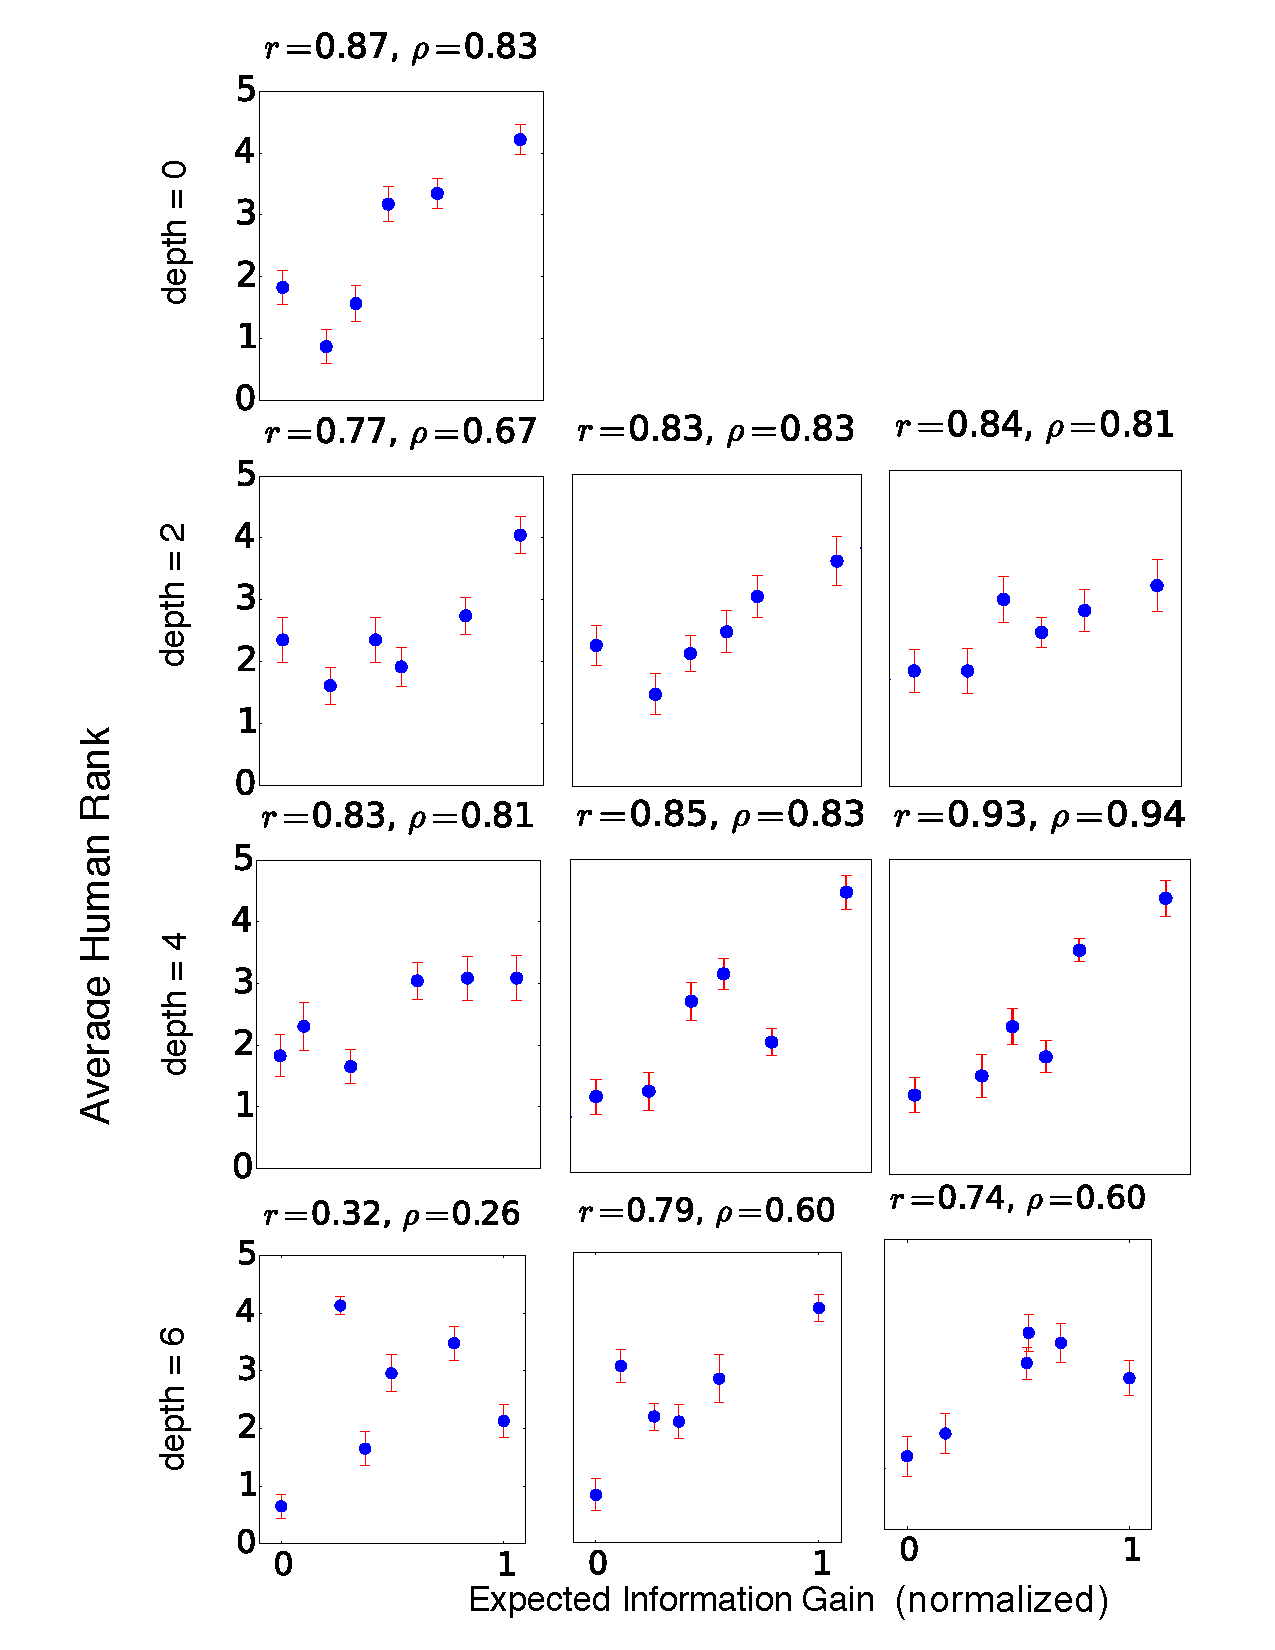
\includegraphics[width=0.7\linewidth]{all_scatterplots}
\end{center}
\caption{Bayesian model fits for one-shot games, with the different games organized by depth. The average human rank score (error bars show $\pm 1$ s.e.) is compared with expected information gain (normalized between 0 and 1).} 
\label{all-trials}
\end{figure}


\begin{figure}[h!]
\begin{center}
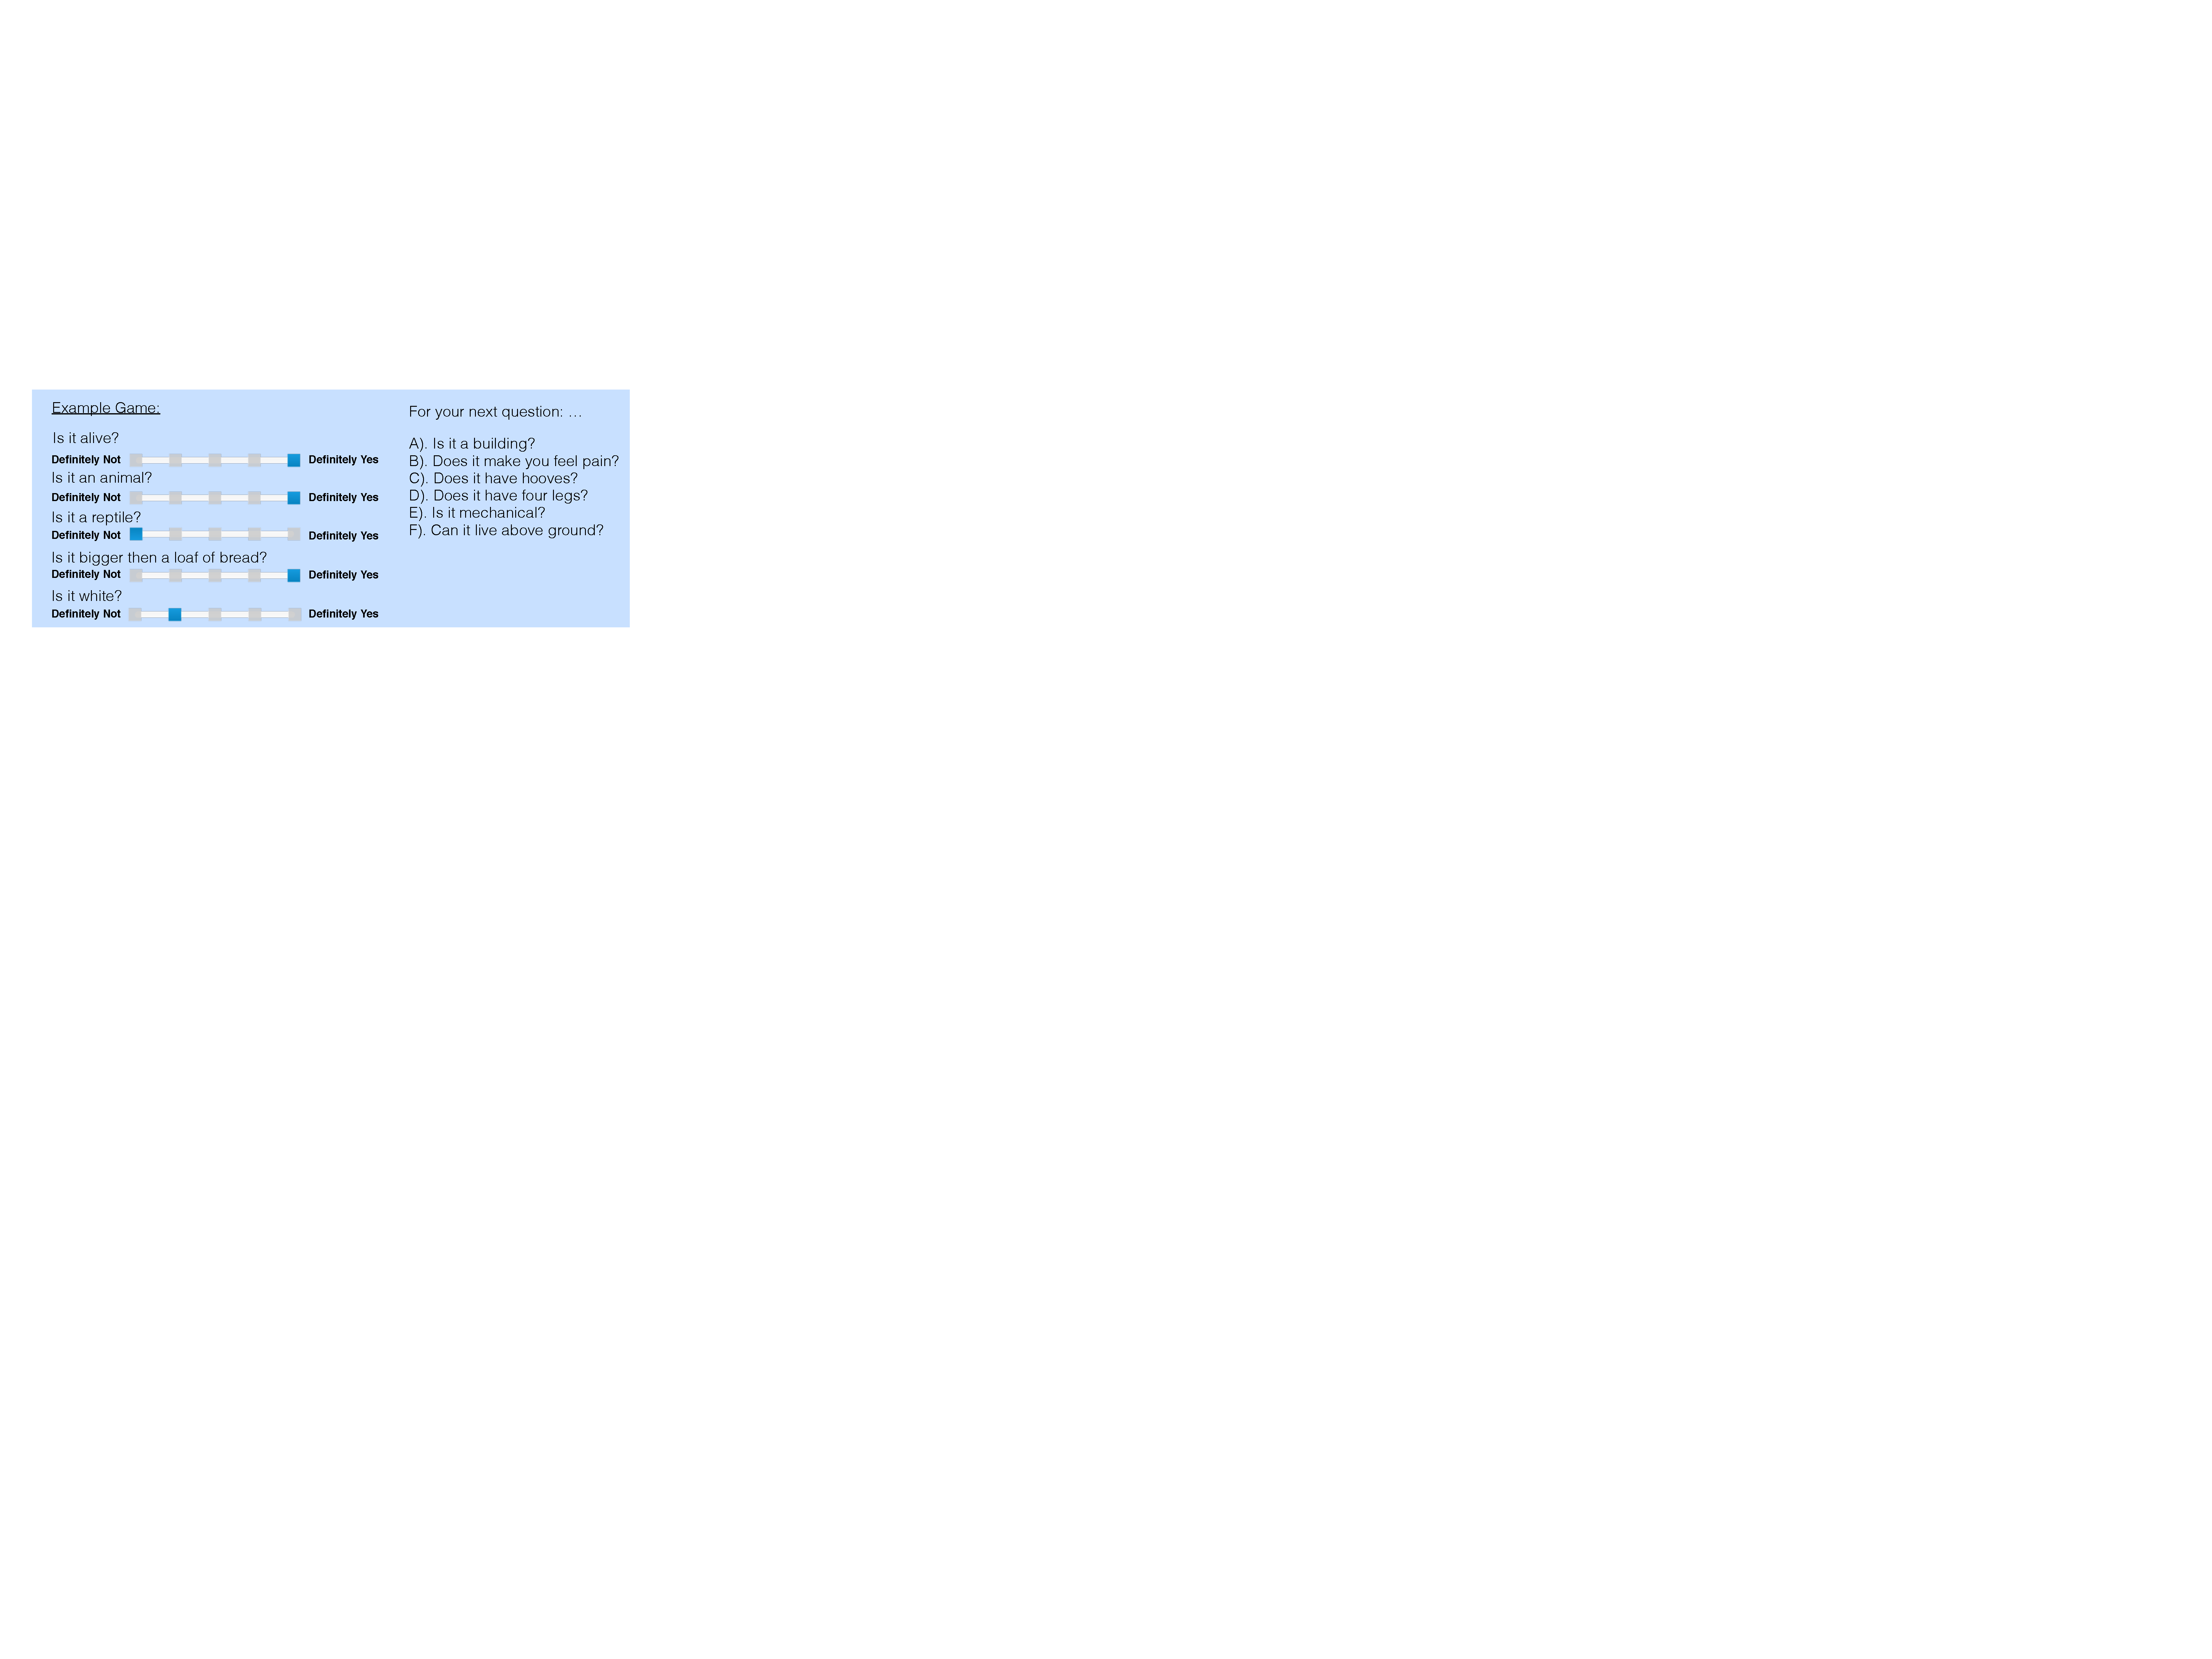
\includegraphics[width=1.0\linewidth]{game_example}
\end{center}
\caption{Example of what a normal game of 20Qs may look like} 
\label{game_example}
\end{figure}

% Ideas for future work: studying question generation, manipulating the prior, exploring more sophisticated noise models, etc.
% serving human-generated games rather than model generated games

\begin{figure}[h!]
\begin{center}
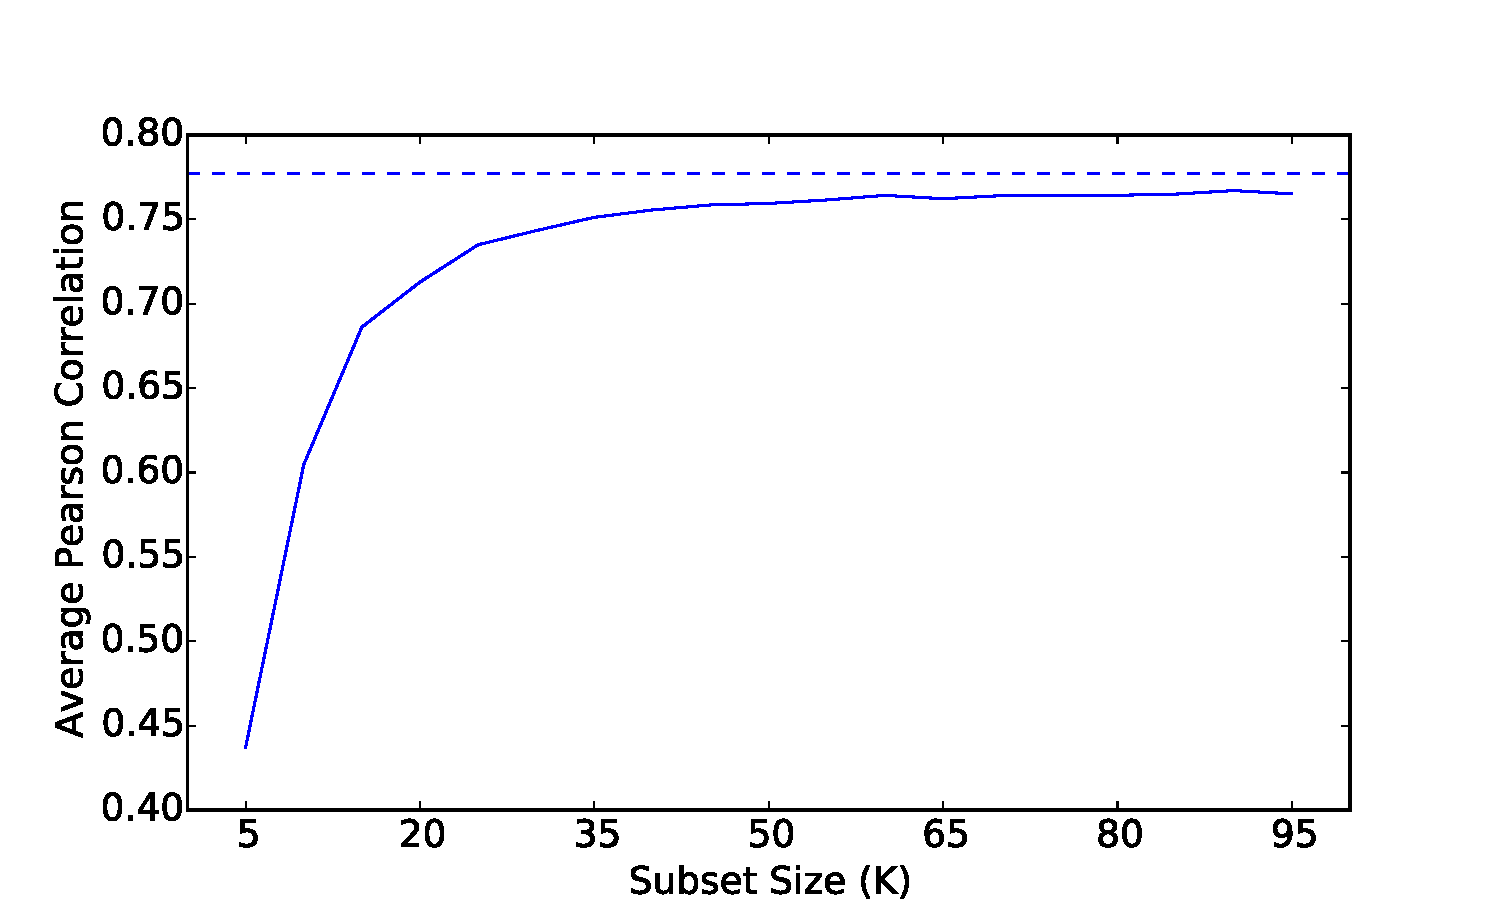
\includegraphics[width=0.85\linewidth]{correlation_for_subset_size}
\end{center}
\caption{Average correlation ($r$) between human preferences on the one-shot games and the Random Subset model for different subset sizes $K$ (solid line; same as Table \ref{table-one-shot} last row). For comparison, the full Bayesian model is shown as the dotted line.}
\label{rs-model-fit}
\end{figure}


\begin{figure}[h!]
\begin{center}
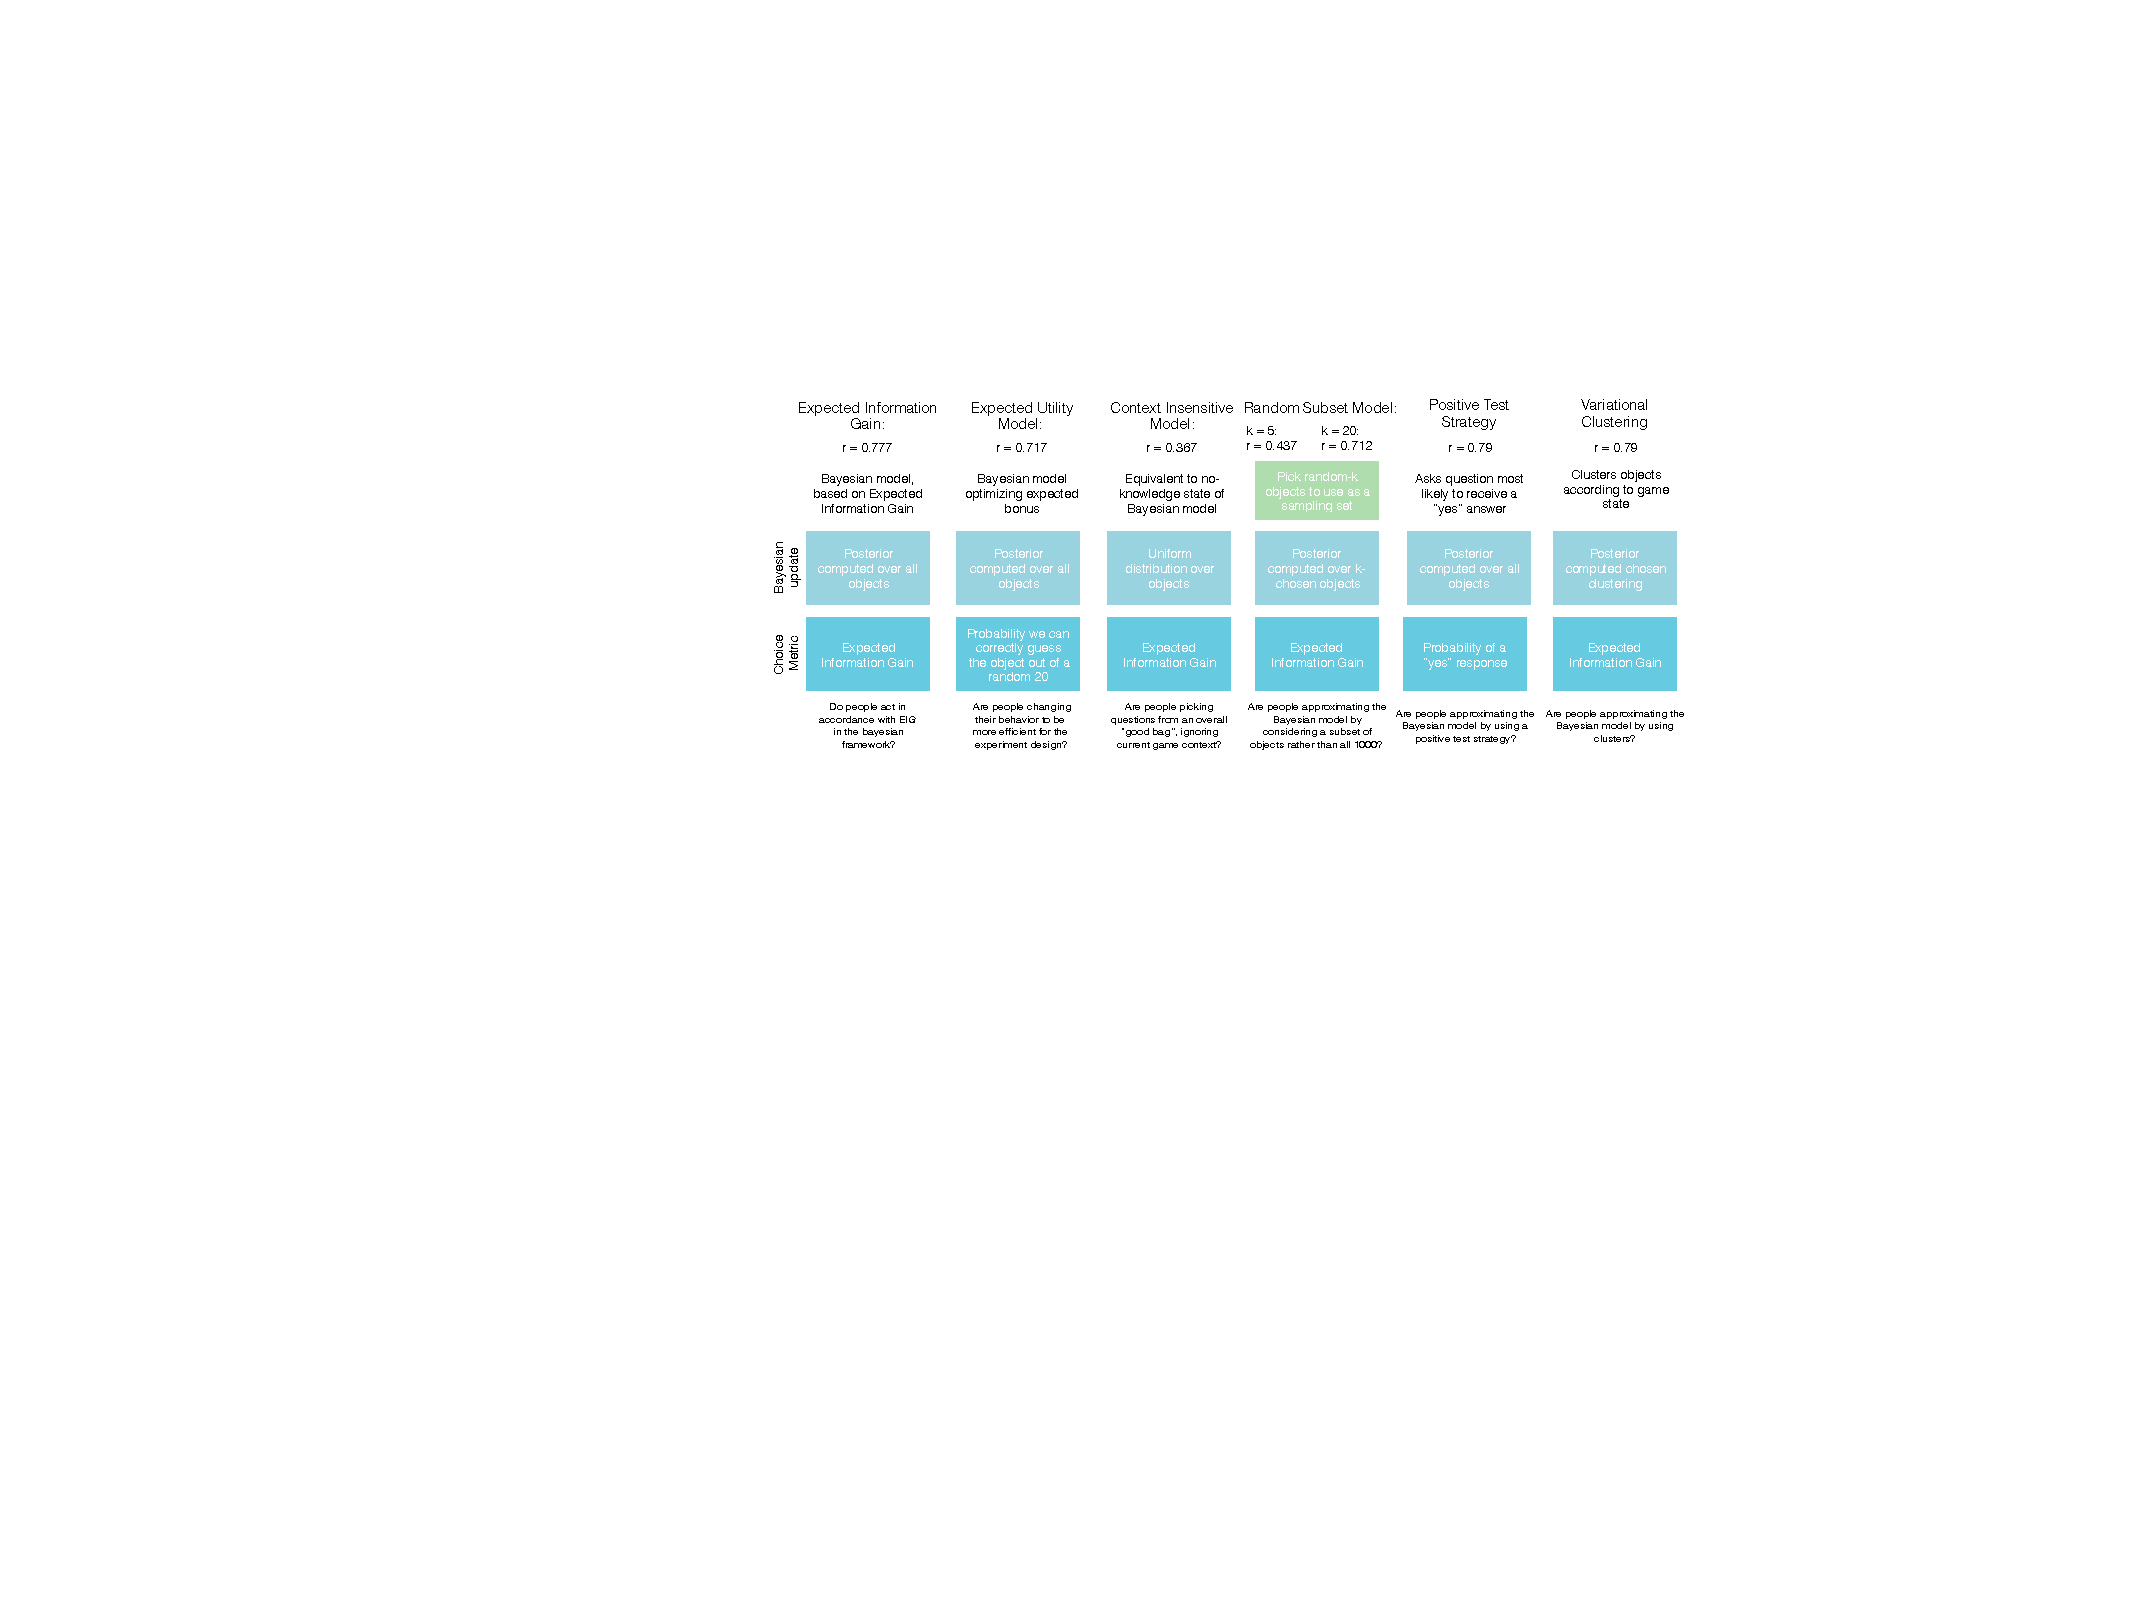
\includegraphics[width=1.0\linewidth]{alternative_models2}
\end{center}
\caption{Differences between each of the alternative models that were tested. All of the models are Bayesian, but they have different steps for computing posteriors and value functions} 
\label{alternative_models_fig}
\end{figure}


\begin{figure}[h!]
\begin{center}
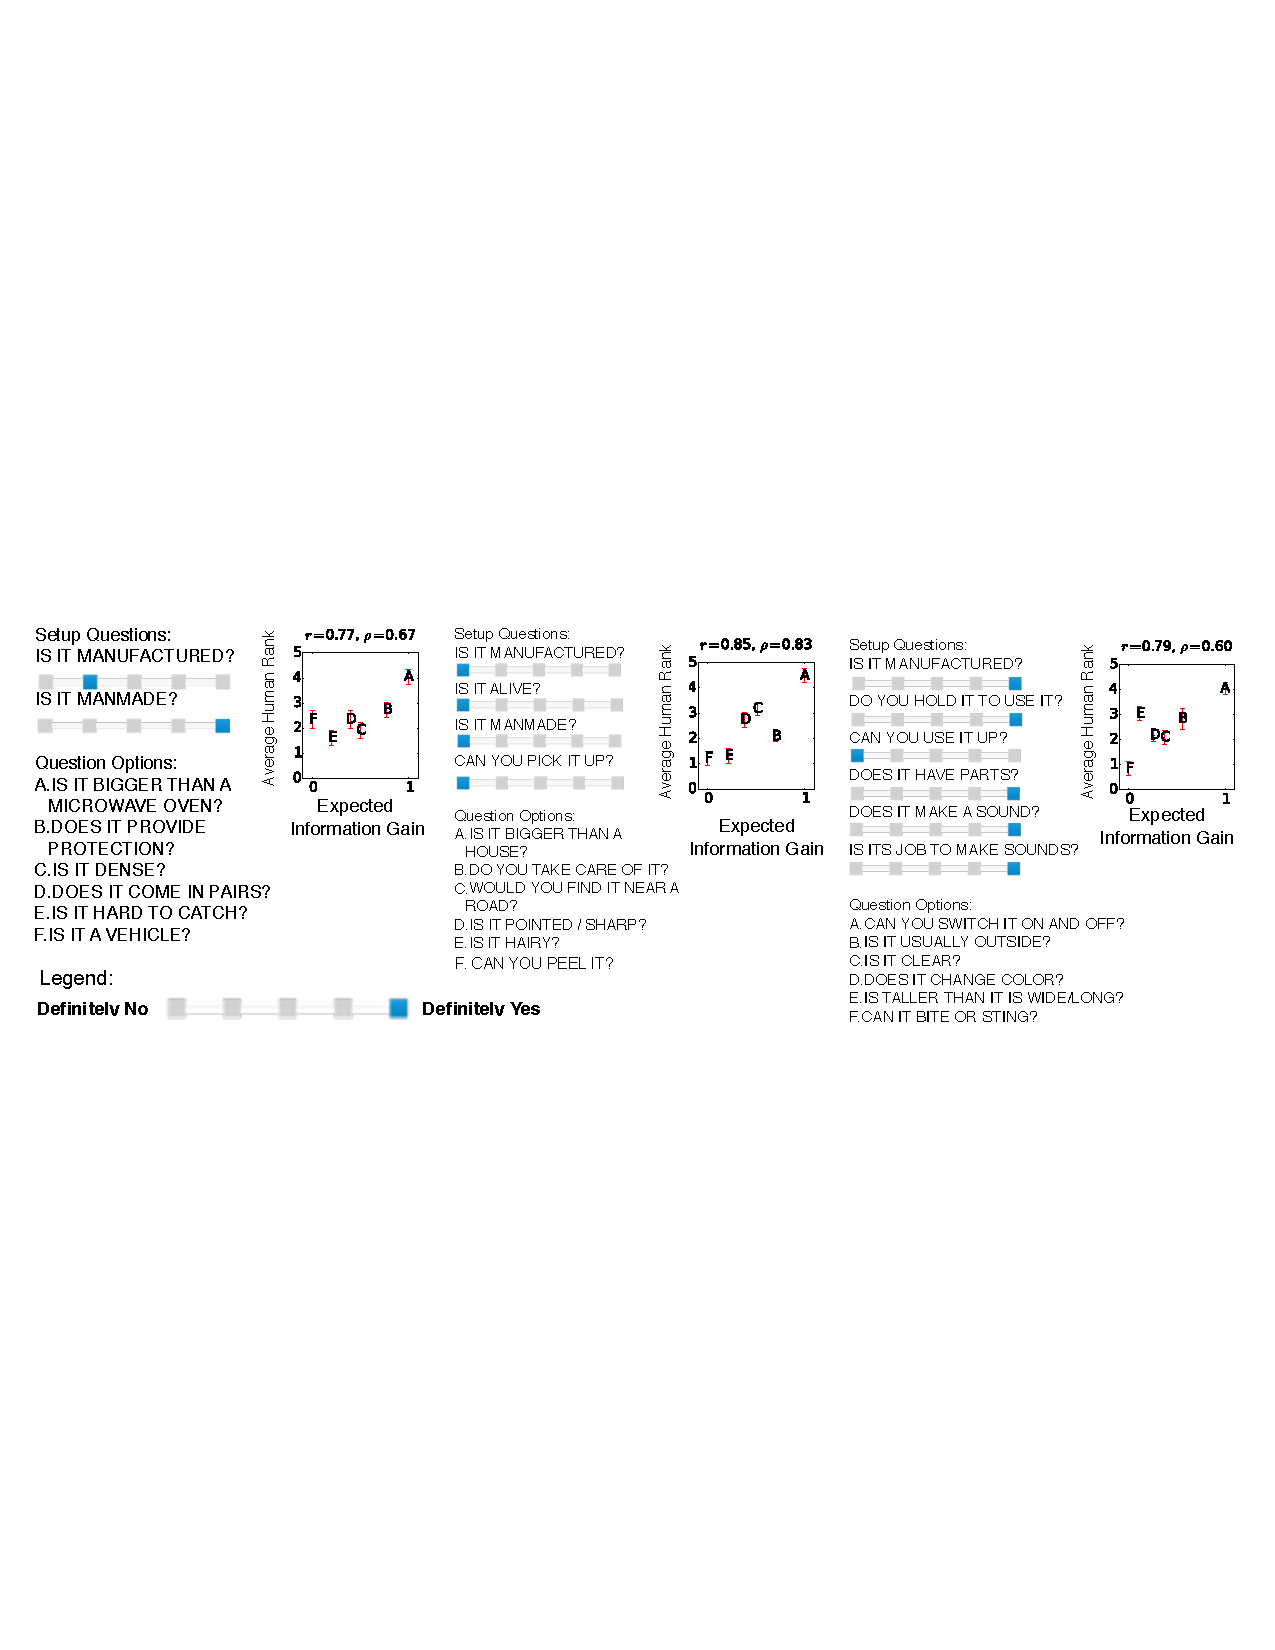
\includegraphics[width=1.0\linewidth]{example_trials}
\end{center}
\caption{Three examples of one-shot 20 question games. Participants observed the Setup Questions with answers on a five point scale (see legend). They then ranked the Question Options in order of preference. In the scatter plots, the average human rank (error bars show $\pm 1$ s.e.) is compared with Bayesian expected information gain, which was normalized to fall between 0 and 1. The object chosen by the game-master for each game were Kitchen, Ground, and Tuba (from left to right).} 
\label{trials-with-questions}
\end{figure}


\begin{figure}[h!]
\begin{center}

\includegraphics[width=0.4\linewidth]{bonus_screen}
\end{center}
\caption{Bonus screen participants are presented with after completion of a full game or oneshot trial} 
\label{bonus_screen}
\end{figure}

\clearpage
\section*{Appendix A.}
Note: this is a rough overview of the algorithm used, documented code can be found in the github link provided in the directory 
``src/models/variational/runner\_variational2.py''. \newline
The posterior probability of a cluster is simply the sum of the probabilities of its children, thus each nodes posterior should it be chosen for the final clustering does not depend on the other elements of the clustering. Similarly, the contribution of that cluster to the total KL divergence is independent of the other elements of the clustering

\begin{equation}
D_{KL}(P||Q) = \sum_o P(o) \log \frac{P(o)}{Q(o)} = 
			\sum_c \sum_{o \in \mc{C}} P(o) (\log P(o) - \log \frac{P(c)}{|\mc{C}|})
\end{equation}

Thus we can define a cost for each cluster such that 
\begin{equation}
J(c) = \sum_{o \in \mc{C}} P(o) (\log P(o) - \log \frac{P(c)}{|\mc{C}|})
\end{equation}
\[
D_{KL}(P||Q) = \sum_c J(c)
\]

The cost of including a node in the final clustering may then be precomputed for each node, and the problem reduced to finding a set of nodes on the tree such that every leaf has exactly one ascendant that is in the clustering. This problem may now be solved using dynamic programming. The subproblem we will adress is finding the optimal way to distribute $k$ clusters among some node and its descendants. If we wish to distribute $k$ clusters among some node $c$ and its descendants, we can either put 1 cluster in the left child and $k-1$ in the right, 2 in the left child and $k-2$ in the right, etc. Solving the problem then comes down to memoizing the optimal way to distribute $k$ clusters among each node $c$, and solving the subproblems exhaustively. The edge case appears either when $k = 1$ or when $c$ is a left. This algorithm was implemented efficiently in Python and was used for the results in this paper.



\vskip 0.2in

\clearpage
\bibliographystyle{apacite}
\setlength{\bibleftmargin}{.125in}
\setlength{\bibindent}{-\bibleftmargin}
\bibliography{20q.bib}

\end{document}